%%%%%%%%%%%%%%%%%%%%%%%%%%%%%%%%%%%%%%%%%%%%%%%%%%%%%%%%%%%%%%%%%%%%%%%%%%%%%%%%
%%%%%%%%%%%%%%%%%%%%%%%%%%%%%%%%%%%%%%%%%%%%%%%%%%%%%%%%%%%%%%%%%%%%%%%%%%%%%%%%
%\documentclass[addpoints,12pt,solution]{exam}
\documentclass[preprint,12pt]{elsarticle}
%% Use the option review to obtain double line spacing

%% Use the options 1p,twocolumn; 3p; 3p,twocolumn; 5p; or 5p,twocolumn
%% for a journal layout:
%% \documentclass[final,1p,times]{elsarticle}
%% \documentclass[final,1p,times,twocolumn]{elsarticle}
%% \documentclass[final,3p,times]{elsarticle}
%% \documentclass[final,3p,times,twocolumn]{elsarticle}
%% \documentclass[final,5p,times]{elsarticle}
%% \documentclass[final,5p,times,twocolumn]{elsarticle}

%% The graphicx package provides the includegraphics command.
\usepackage{graphicx}
%% The amssymb package provides various useful mathematical symbols
\usepackage{amssymb}
\usepackage{amsmath}
\usepackage{titlesec}
\usepackage{breqn}
\usepackage{chemfig}
\usepackage{csvsimple}
\usepackage{tfrupee}  
%% The amsthm package provides extended theorem environments
%% \usepackage{amsthm}

%% The lineno packages adds line numbers. Start line numbering with
%% \begin{linenumbers}, end it with \end{linenumbers}. Or switch it on
%% for the whole article with \linenumbers after \end{frontmatter}.
\usepackage{lineno}
\usepackage{natbib}
\usepackage{hyperref}
% \usepackage[top=0.75in, bottom=0.75in, left=0.55in, right=0.85in]{geometry}
\usepackage{graphicx}
\usepackage{url}
\usepackage{palatino}
\usepackage{tabularx}
\usepackage{graphicx}
\usepackage{multicol}
\usepackage{graphicx}
\usepackage{amssymb}
\usepackage{float}
\usepackage{amsmath}
\usepackage{rotating}
\usepackage{subfigure}
\usepackage{multirow}
\usepackage{mathrsfs}
\usepackage{xfrac}
\usepackage[font=small,skip=0pt]{caption}
%\usepackage[numbers,sort&compress]{natbib}
%\usepackage{hyperref}
\usepackage{pgf,tikz}
\usetikzlibrary{shapes,arrows,chains}
\usetikzlibrary[calc]
\usepackage{graphicx}
\graphicspath{ {./images/}}
\usepackage{geometry}
\geometry{lmargin=1in,rmargin=1in,tmargin=1in,bmargin=1in}
\usepackage{lipsum}
%\pagestyle{empty}
\usepackage{natbib}
\pagenumbering{arabic}
%\usepackage[T1]{fontenc}
\usepackage{setspace}
\usepackage{mathptmx}
\usepackage{t1enc}
%\usepackage{xkeyval}
%\usepackage{chemformula}
%\usepackage{array}
%\usepackage{booktabs}
%\usepackage{hypdoc}
%\usepackage{listings}
%\usepackage{lmodern}
%\usepackage{mathpazo}
%\usepackage{microtype}
\usepackage{graphicx}
\usepackage{amssymb}
\usepackage{float}
\usepackage{amsmath}
\usepackage{rotating}
\usepackage{subfigure}
\usepackage{multirow}
\usepackage{xfrac}
\usepackage[font=small,skip=0pt]{caption}
%\usepackage[numbers,sort&compress]{natbib}
%\usepackage{hyperref}
\usepackage{pgf,tikz}
\usetikzlibrary{shapes,arrows,chains}
\usetikzlibrary[calc]
\usepackage{graphicx}
\usepackage{geometry}
\geometry{lmargin=1in,rmargin=1in,tmargin=1in,bmargin=1in}
\usepackage{lipsum}
%\pagestyle{empty}
\usepackage{natbib}
\pagenumbering{arabic}
%\usepackage[T1]{fontenc}
\usepackage{setspace}
\usepackage{mathptmx}
\usepackage{t1enc}
%\usepackage{xkeyval}
%\usepackage{chemformula}
%\usepackage{array}
%\usepackage{booktabs}
%\usepackage{hypdoc}
%\usepackage{listings}
%\usepackage{lmodern}
%\usepackage{mathpazo}
%\usepackage{microtype}
\usepackage{lineno,hyperref}
\usepackage{multirow}
\usepackage{cancel}
\usepackage{url}
\usepackage[norule]{footmisc}
\usepackage[utf8]{inputenc}
\usepackage[english]{babel}
\hypersetup{colorlinks = true,linkcolor = blue,urlcolor = blue}
% \fontfamily{SansSerif}
% \selectfont
% \usepackage[T1]{fontenc}
% \usepackage
%% natbib.sty is loaded by default. However, natbib options can be
%% provided with \biboptions{...} command. Following options are
%% valid:
%%   round  -  round parentheses are used (default)
%%   square -  square brackets are used   [option]
%%   curly  -  curly braces are used      {option}
%%   angle  -  angle brackets are used    <option>
%%   semicolon  -  multiple citations separated by semi-colon
%%   colon  - same as semicolon, an earlier confusion
%%   comma  -  separated by comma
%%   numbers-  selects numerical citations
%%   super  -  numerical citations as superscripts
%%   sort   -  sorts multiple citations according to order in ref. list
%%   sort&compress   -  like sort, but also compresses numerical citations
%%   compress - compresses without sorting
%%
%% \biboptions{comma,round}
% \biboptions{}
\usepackage{caption}
\usepackage{caption}
\usepackage{algorithm} 
\usepackage[noend]{algpseudocode}
\usepackage{amsmath}
\DeclareMathOperator*{\argmin}{argmin}
\DeclareMathOperator*{\argmax}{argmax}
\newcommand*{\argminl}{\argmin\limits}
\newcommand*{\argmaxl}{\argmax\limits}

\let\orupee\rupee
\def\rupee{\ifmmode\text{\orupee}\else\orupee\fi}


\begin{document}


\hrule
\vspace{1mm}
\noindent 
\begin{center}
{\Large MA5895 : Numerical Optimization} \\

{\large Combined Assignment Report} \\
{\large Cell Tower Problem   \hfill }
\end{center}
\vspace{1mm}
\noindent 


\titleformat{\section}
{\normalfont\fontfamily{phv}\fontsize{17}{20}\bfseries\itshape}{\thesubsection}{1em}{}

\titleformat{\subsection}
{\normalfont\fontfamily{phv}\fontsize{13}{17}\bfseries\itshape}{\thesubsection}{1em}{}

%%%%%%%%%%%%%%%%%%%%%%%%%%%%%%%%%%%%%%%%%%%%%%%%%%%%%%%%%%%%%%%%
% Enter name and roll number here
\noindent {\bf Name:} Pragnesh Rana \hfill {\bf Roll number:} ME17S301
%%%%%%%%%%%%%%%%%%%%%%%%%%%%%%%%%%%%%%%%%%%%%%%%%%%%%%%%%%%%%%%%%%
\vspace{2mm}
\hrule
\vspace{2mm}
{\small

\textbf{Summary : } Hi

}
\vspace{2mm}
\hrule

%%
%% Following citation commands can be used in the body text:
%% Usage of \cite is as follows:

%%   \cite{key}          ==>>  [#]
%%   \cite[chap. 2]{key} ==>>  [#, chap. 2]
%%   \citet{key}         ==>>  Author [#]

\tableofcontents

\section{Problem Statement}
In city planning, the issue is to find out optimal cites out to plant the towers for given the population and budget constrain. To solve the problem, divide the population into small region based on maximum capacity to plant the cell tower. Each site location may also cover other specified number of locations. Out of all possible cell tower cites, find out the optimal locations which can serve maximum  population keeping control over budget.

\newpage

\section{Assumptions}
Assumed that,
\begin{itemize}
	\item The city is a rectangular region
	
	\item One region can be covered by more than one cell tower as they might have different frequency.
	
	\item The cost of each tower is assumed as $30,00,000~\rupee$ \cite{cost} and other cost is 10$\%$ times the population covered by each network(self+neighboring region).
	
	\item Each cellular location(centroid) can cover 3 neighboring region apart from covering its own region.
	
	(Can be easily changed but in whole analysis kept fixed)
	\item The euclidean distance is used for measuring distance. 
	
	\item The resultant location of cell cite is average value of centroids(centroid of covered regions).
	
\end{itemize}


\section{Formulation} \label{sec:formulation}
The formulation of problem is divided into two parts.
\begin{enumerate}
\item \textbf{Clusters from population data }

The population is divided into K-clusters using k-means algorithm given number potential cites to plant the cell towers. The partition is made such that each person belong to cluster with nearest possible mean location or generate K-clusters with minimized the within-cluster sum of squares(variance).\ref{wikiKmeans}.

The objective function for clustering is defined as\cite{wikiKmeans},

\begin{equation}
J = \argmin_s \sum_{i=1}^{k} \sum_{x\in s_i} ||x - C_i ||^2
\end{equation}

where,
\begin{itemize}
	\item $\mu_i$ = mean of points $s_i$
	\item $s$ = Population sets ${s_1,s_2,..,s_k} $
	\item $C_i$ = $i^{th}$ cluster
	\item k = Total required clusters
\end{itemize}

\item \textbf{Optimal location of sites}

After obtaining all the clusters, now objective is to find out the optimum locations which can cover maximum location keeping control over budget. The formulation of problem is instance of  mixed integer programming(MIP)\cite{maximal}.

The formulation is given as,
\begin{equation}
	\begin{aligned}
\text{Maximize} \hspace{2mm} Z &= \sum_{j \in R} p_j \cdot y_j \\
\text{S.T,} \hspace{3mm}\sum_{(i,j)} x_i &\geq y_j \hspace{3mm} \forall j \in \mathcal{R} \\
\sum_{i \in T} c_i \cdot x_i &\leq \text{Budget}
\end{aligned}
\end{equation}

where,
\begin{itemize}
	\item j - Index of regions $\in R$
	\item i - Index of optimal sites to build tower $\in T$
	\item T - Set of potential sites
	\item R - Set of regions
	\item $c_i$ - Cost of setting up a tower at site-i
	\item $p_j$ - Population at region-j
	\item $y_j$ - Binary variable for assignment of region \{1 if region is covered else 0\}
	\item $x_i$ - Binary variable for tower  \{1 if tower  is build else 0\}
\end{itemize}

\subitem \textbf{In Words:}
The objective function is to maximize total covered population with constrain that each region is covered by at least one tower (constrain-1) ensuring the total cost do not exceed the budget(constrain-2).

\end{enumerate}




The MIP(Mixd Interger Programming) problem is solved  linear-programming based branch-and-bound algorithm\cite{gurobiSol}. The solution is implemented using python base package of gurobi (academic version)\cite{gurobi}.  


 
\section{Approach to tackle the problem}

\begin{itemize}
	\item In specified rectangular region, using limit of region population is generated by 5 blobs with appropriate $sigma$ such that spread is enough to cover enough region and 10$\%$ of the population is randomly spread over given region.
	\item In Fundamental of cellular network\cite{david} it was mentioned that cellular network region can be approximated by hexagon so, the whole population is divided into given number small regions(cluster) using k-means algorithm which follows shapes of polygon(Approximation of pentagon and hexagon.)
	\item It was also mentioned that tower near to each other does not have same frequency so, overlapping of frequency in one region may not be an issue\cite{david}. In simulation, the tower located an the centroid of one region can cover three nearest regions.
	
	\item Once all the regions is obtained, centroid of each region denotes potential cite to plant the cell tower.
	
	\item Out of all potential cites the optimal sites are obtained such that it can cover the maximum population given budget constrain.
	
	\item This problem is another example of maximal covering location problem\cite{maximal}and set cover problem. The mathematical formulation of problem is given in section-\ref{sec:formulation} in the form of Mixed Integer Programming(MIP).
	
	\item The solution of the problem is  obtained by Gurobi Optimizer python based package. Further detail is given in section-\ref{sec:formulation}.
	
	\item Let's take an example,
	Input:
	\subitem Total Population = 100000
	\subitem Count of Covering Region = 4 (self+3 Neighbor)
	\subitem Maximum Capacity to Plant Towers or Total regions = 12 
	\subitem Cost per each tower = $30,00,000~\rupee$
	\subitem Total budget = 10,00,000 * MAX Capacity = $1,20,00,000~\rupee$
	
	\item Whole population is divided into 12 clusters as given in fig.-\ref{vor12}. Each cluster centroid is a potential cite for the final cell location. But to find out optimal location of sites with specified constrain \ref{eq:constrain}, the problem is solved using gorubi solver which works based on maximum covering location algorithm with mixed integer programming. 
	

	
		Running the simulation using aforementioned parameters, the obtained result is given as below,
		
		\begin{figure}[H]
			\centering  
			\subfigure[Voronoi Diagram]
			{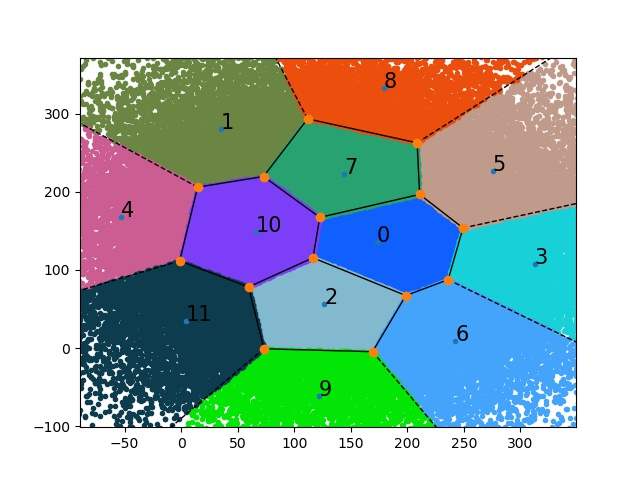
\includegraphics[width=0.43\linewidth]{./12Regions.jpg}\label{vor12}}
			\subfigure[Final cites to plant towers]
			{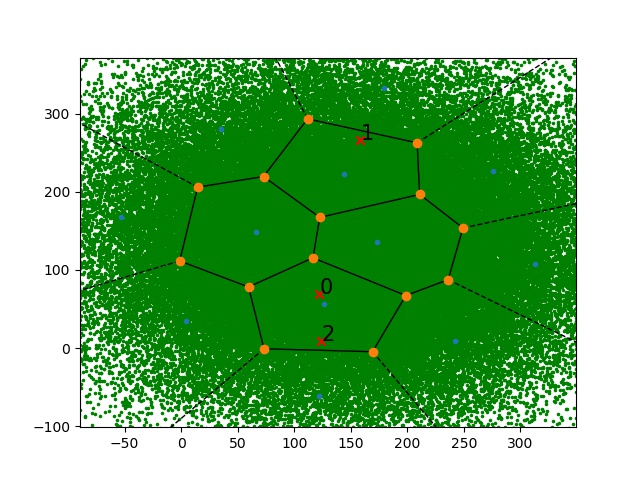
\includegraphics[width=0.43\linewidth]{./12FinalResult.jpg}\label{cites12}}
			\caption{Fig.-\ref{vor12} shows voronoi diagram obtained by diving the whole population into cluster using K-Means algorithm and Fig.-\ref{cites12} shows the final cites to plant the towers (By RED MARKED DOTS).}
			\label{fig:for12}
		\end{figure}
		
		\begin{table}[H]
			\centering
			\scalebox{0.61}{
				\begin{tabular}{|l|l|l|l|l|l|l|l|l|l|l|l|l|l|}
					\hline
					\textbf{Region} & 0 & 1 & 2 & 3 & 4 & 5 & 6 & 7 & 8 & 9 & 10 & 11 & Total \\ \hline
					\textbf{Population} & 44369 & 6539 & 11246 & 7466 & 4998 & 7909 & 8601 & 10757 & 4503 & 4743 & 12511 & 6898 & 130000 \\ \hline
					\textbf{Cost to build (Lakhs $\rupee $)} & 3034514 & 3028266 & 3061623 & 3060339 & 3025948 & 3062592 & 3023455 & 3061383 & 3025205 & 3026205 & 3066372 & 3028755 & 30418113 \\ \hline
					\multicolumn{13}{|r|}{\textbf{Budget}} & 12013000 \\ \hline
				\end{tabular}
		}
		\vspace{1mm}
		\caption{Summary of Population and cost associated with each region along with avialble budget. }
		\label{tab:summary}
		\end{table}
		
			\begin{table}[H]
				\centering
				\begin{tabular}{|c|c|c|c|}
					\hline
					\textbf{RegionCenter} & \textbf{NeighborCenter0} & \textbf{NeighborCenter1} & \textbf{NeighborCenter2} \\ \hline
					0 & 7 & 2 & 10 \\ \hline
					1 & 7 & 10 & 4 \\ \hline
					2 & 0 & 10 & 9 \\ \hline
					3 & 6 & 5 & 0 \\ \hline
					4 & 10 & 1 & 11 \\ \hline
					5 & 3 & 7 & 0 \\ \hline
					6 & 3 & 2 & 9 \\ \hline
					7 & 0 & 10 & 8 \\ \hline
					8 & 7 & 5 & 1 \\ \hline
					9 & 2 & 6 & 11 \\ \hline
					10 & 0 & 7 & 2 \\ \hline
					11 & 2 & 10 & 4 \\ \hline
				\end{tabular}					\vspace{1mm}
				\caption{Table of centroid and its three nearest centroid index}
				\label{tab:centeroids}
			\end{table}
		
	\item Centroid and its three nearest neighbor centroid is given in table-\ref{tab:centeroids} which indicates if cell tower is planted on specific region center, it can cover regions with three nearest centroid along with its own region. The objective is to find out the best possible sites which can cover maximum population with restriction of budget. For example if cell tower is planted at centroid location-0 then it can cover region with centroid location 7, 2, and 10,which can be verified from figure-\ref{vor12}.
	
	\item The problem has been solved by running the algorithm considering specified constrain and result is given in fig-\ref{cites12}. The centroid 2,8 and 9 are resultant place obtained by algorithm.
	
	\item The tower at centroid location-2 can cover region 2,0,10,9. Likewise, tower at location 8 and 9 region can cover regions 8,7,5,1 and 9,2,6,11.
	
	\item As location 2 can cover regions-2,0,10 and 9 , so final location of cell site is obtained by taking average value coordinates of centroids.
	
	\item It is observed that the region 2 and 9 are covered twice. The region 4 and 3 are not covered due to budget constrain.
	
	\item Overall, 86.95\% population is covered using 75.94\% budget.
	 

	
	
	
	
	
	
	
\end{itemize}


\section{Algorithm}
Hello





\section{Results and Discussion}
hello
\subsection{Result with few values of input}

\subsection{Computational time as a function of input parameters}
\subsection{Largest problem solution}









	\newpage
	
\section{References}
	%%
	%% Following citation commands can be used in the body text:
	%% Usage of \cite is as follows:
	
	%%   \cite{key}          ==>>  [#]
	%%   \cite[chap. 2]{key} ==>>  [#, chap. 2]
	%%   \citet{key}         ==>>  Author [#]
	
	%% References with bibTeX database:
	\bibliographystyle{ieeetr}
	\bibliography{biblio.bib}					
	%% Authors are advised to submit their bibtex database files. They are
	%% requested to list a bibtex style file in the manuscript if they do
	%% not want to use model1-num-names.bst.
	
	%% References without bibTeX database:
	
	% \begin{thebibliography}{00}
	
	%% \bibitem must have the following form:
	%%   \bibitem{key}...
	%%
	
	% \bibitem{}
	
	% \end{thebibliography}


\end{document}